\documentclass{beamer}
\usecolortheme{wolverine}

% math stuff
\usepackage{amsmath}
\usepackage{amsthm}
\usepackage{amssymb}
\usepackage{xcolor}

\usepackage{float}
\usepackage{subcaption}

% to insert images
\usepackage{graphicx}

% to correctly insert stressed characters
\usepackage[T1]{fontenc}
\usepackage[utf8]{inputenc}

\usepackage{multirow}

% Bibliography
\usepackage[style=alphabetic]{biblatex}
% \usepackage[nottoc]{tocbibind}
\usepackage{bibentry}
\setcounter{biburllcpenalty}{9000}
\usepackage{nameref}
\addbibresource{source.bib}

% to put links in table of contents
\usepackage{hyperref}
\hypersetup{colorlinks=false, %set true if you want colored links
    linktoc=all,     %set to all if you
}

% Add symbols
% \usepackage{textcomp}

% Add command for Real and Z sets
% \usepackage{dsfont}
% \newcommand{\Rset}{$\mathds{R}$}
% \newcommand{\Zset}{$\mathds{Z}$}

% Code highlighting
% \usepackage{minted}
% \usemintedstyle{perldoc}
% \setminted{
%     frame=single,
%     breaklines,
% }

% tikz figures
% \usepackage{tikz}
% \input{style.tikzstyle}
% \usetikzlibrary{positioning}

% number rounding
\usepackage{siunitx}
\sisetup{round-mode=places,round-precision=5}

\definecolor{myyellow}{RGB}{225, 225, 0}

\title{Thesis notes}
\date{23rd March}

% any code between @(...)@ is escaped back to LaTeX
% \lstset{escapeinside={@(}{)@}}

% algorithms
\usepackage[ruled,vlined]{algorithm2e}

\begin{document}
\frame{\titlepage}

\begin{frame}[c]
    \frametitle{Detecting controversial content}
    \begin{figure}
        \begin{center}
            \begin{subfigure}[b]{0.4\textwidth}
                \centering
                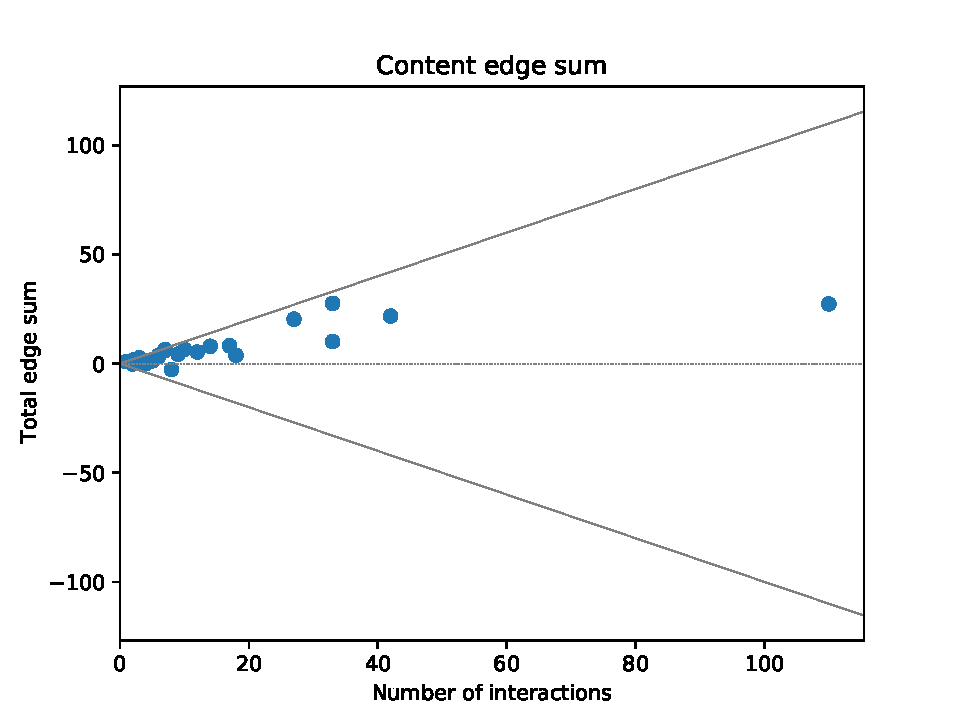
\includegraphics[width=\textwidth]{out/bbcscience200/edge-sum-n-interactions.pdf}
                \caption{@bbcscience}
                \label{fig:out/bbctech200/edge-sum-n-interactions.pdf}
            \end{subfigure}
            \begin{subfigure}[b]{0.4\textwidth}
                \centering
                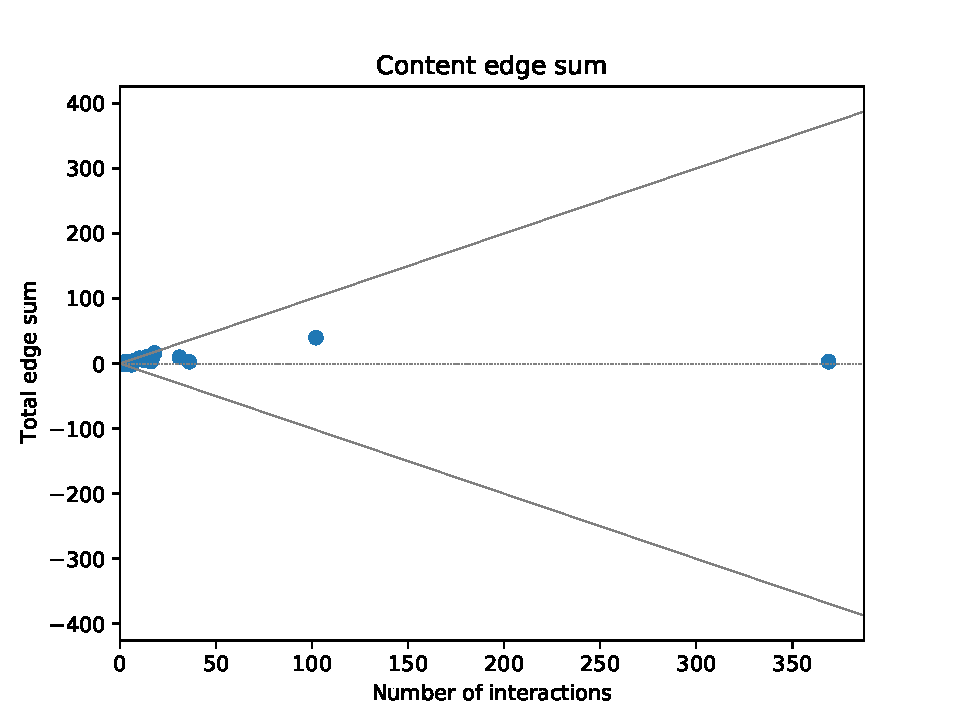
\includegraphics[width=\textwidth]{out/bbctech200/edge-sum-n-interactions.pdf}
                \caption{@bbctech}
                \label{fig:out/bbctech200/edge-sum-n-interactions.pdf}
            \end{subfigure}
            \begin{subfigure}[b]{0.4\textwidth}
                \centering
                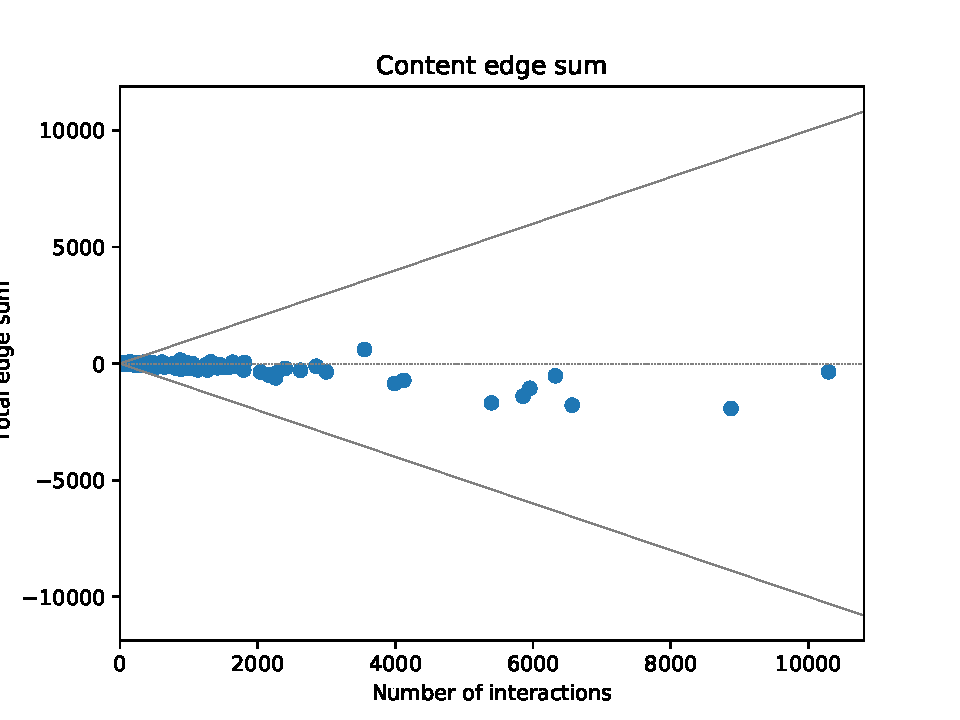
\includegraphics[width=\textwidth]{out/foxnews400/edge-sum-n-interactions.pdf}
                \caption{@foxnews}
                \label{fig:out/foxnews400/edge-sum-n-interactions.pdf}
            \end{subfigure}
            \begin{subfigure}[b]{0.4\textwidth}
                \centering
                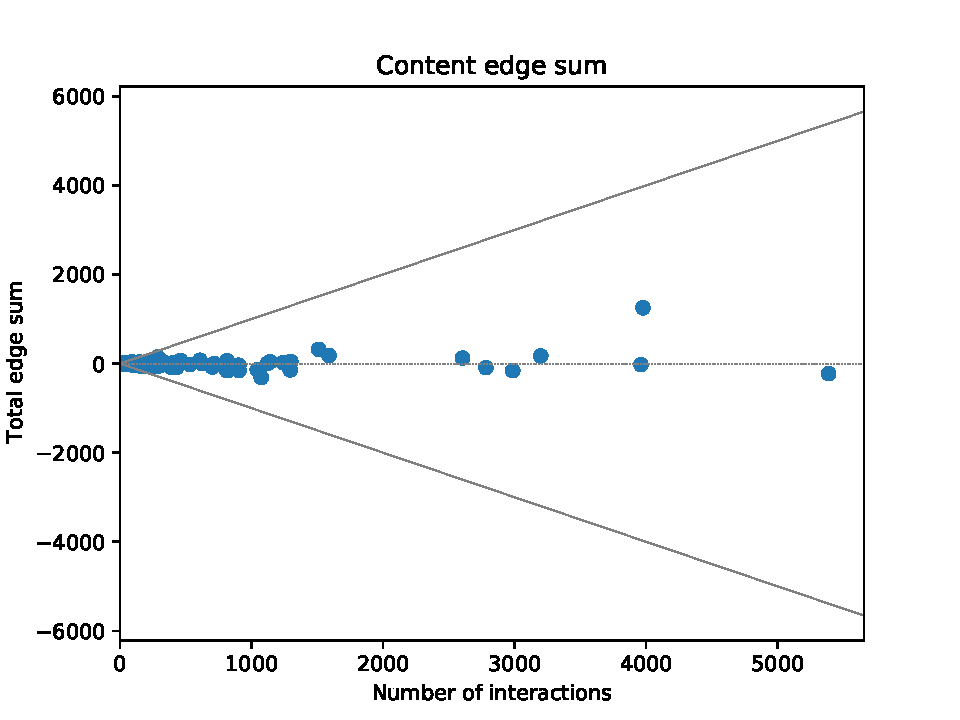
\includegraphics[width=\textwidth]{out/politics200/edge-sum-n-interactions.pdf}
                \caption{r/politics}
                \label{fig:out/politics200/edge-sum-n-interactions.pdf}
            \end{subfigure}
        \end{center}
        \caption{edge sum over number of interactions}
    \end{figure}
\end{frame}


\begin{frame}[c]
    \frametitle{Detecting controversial content}
    \begin{figure}
        \begin{center}
            \begin{subfigure}[b]{0.4\textwidth}
                \centering
                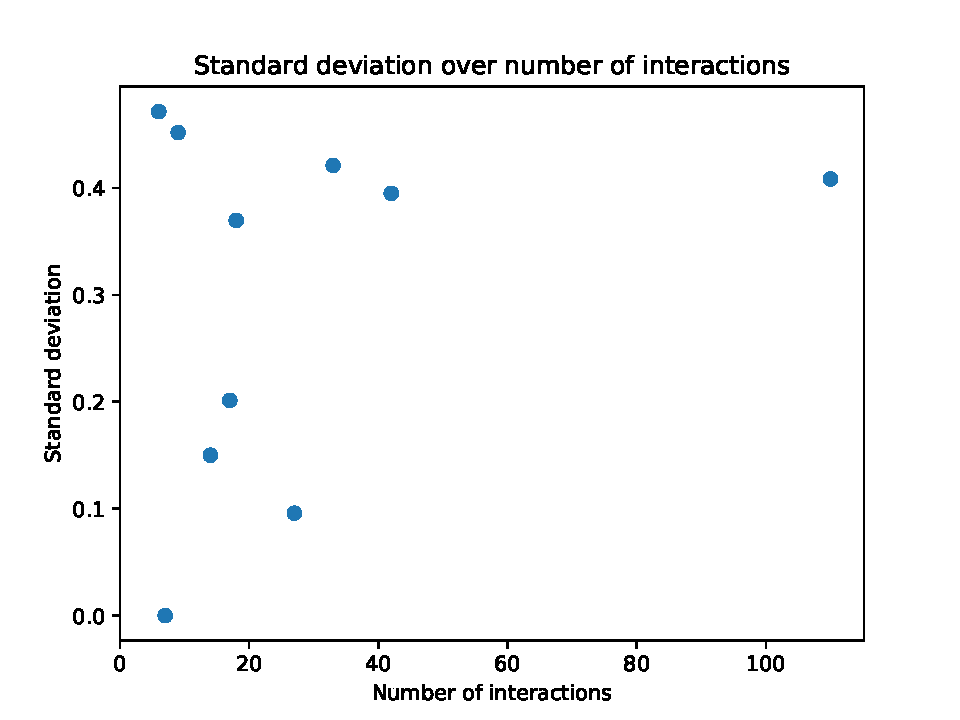
\includegraphics[width=\textwidth]{out/bbcscience200/std-dev-n-interactions.pdf}
                \caption{@bbcscience}
                \label{fig:out/bbctech200/std-dev-n-interactions.pdf}
            \end{subfigure}
            \begin{subfigure}[b]{0.4\textwidth}
                \centering
                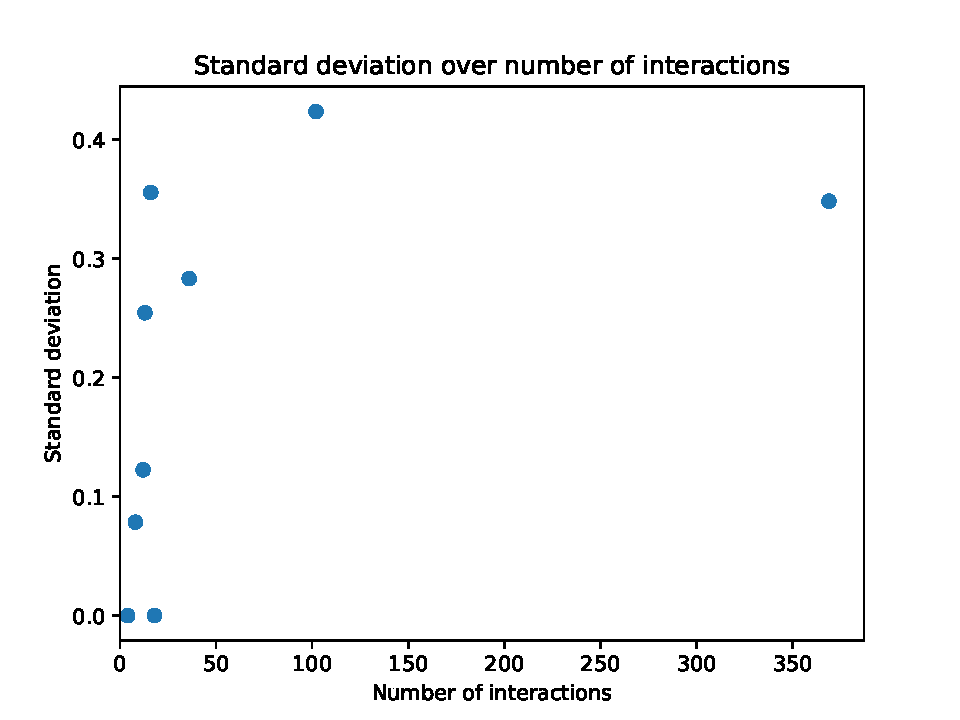
\includegraphics[width=\textwidth]{out/bbctech200/std-dev-n-interactions.pdf}
                \caption{@bbctech}
                \label{fig:out/bbctech200/std-dev-n-interactions.pdf}
            \end{subfigure}
            \begin{subfigure}[b]{0.4\textwidth}
                \centering
                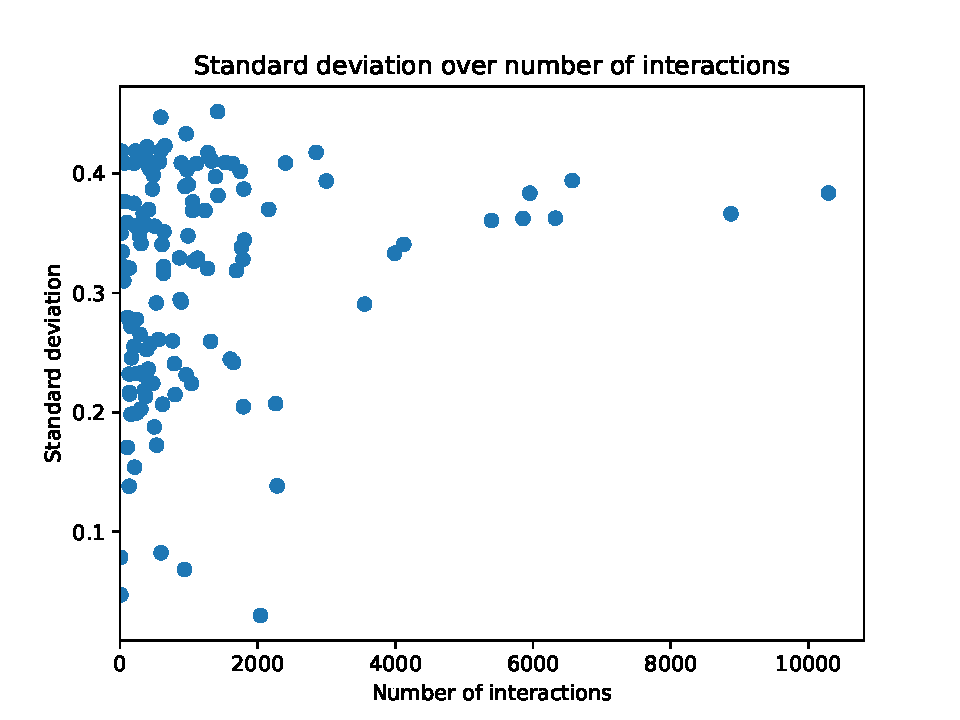
\includegraphics[width=\textwidth]{out/foxnews400/std-dev-n-interactions.pdf}
                \caption{@foxnews}
                \label{fig:out/foxnews400/std-dev-n-interactions.pdf}
            \end{subfigure}
            \begin{subfigure}[b]{0.4\textwidth}
                \centering
                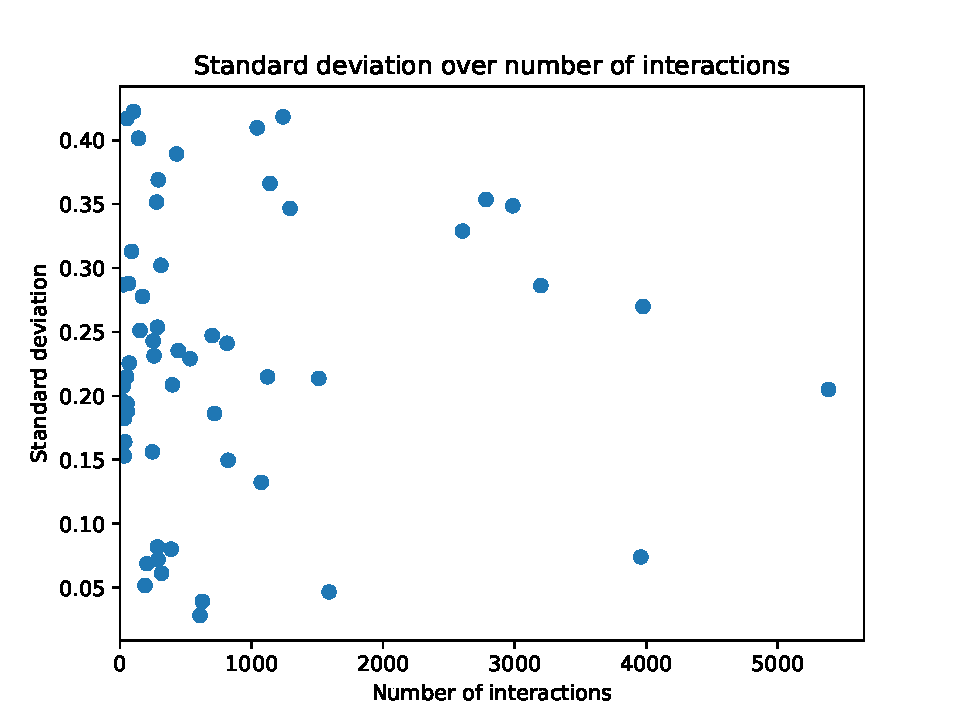
\includegraphics[width=\textwidth]{out/politics200/std-dev-n-interactions.pdf}
                \caption{r/politics}
                \label{fig:out/politics200/std-dev-n-interactions.pdf}
            \end{subfigure}
        \end{center}
    \end{figure}
\end{frame}


% \begin{frame}[c]
%     \frametitle{Detecting controversial content}
%     \begin{figure}
%         \begin{center}
%             \begin{subfigure}[b]{0.4\textwidth}
%                 \centering
%                 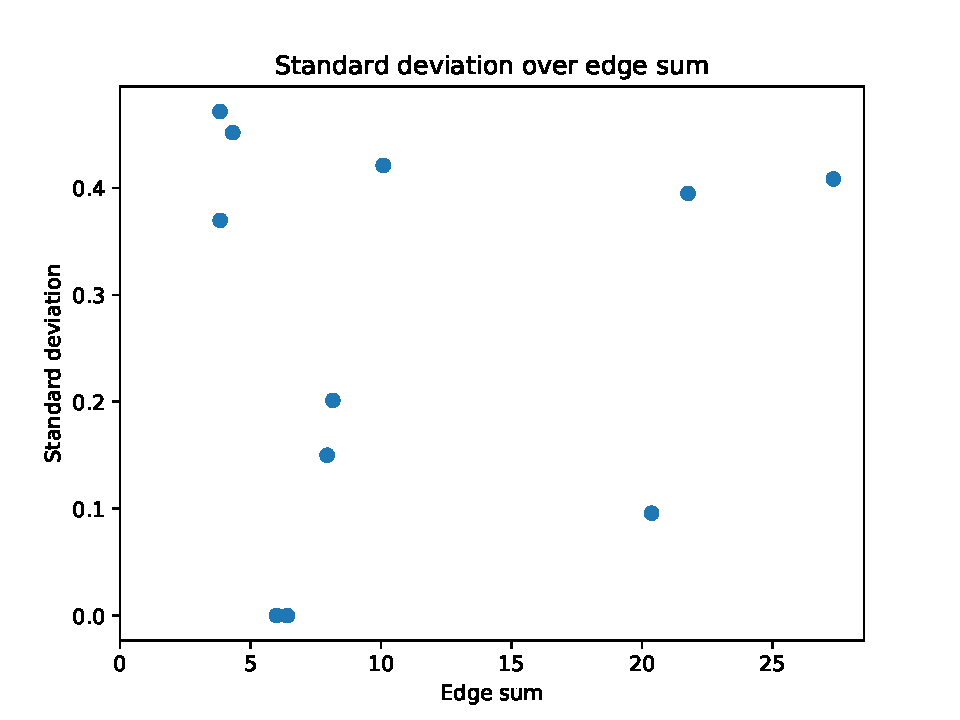
\includegraphics[width=\textwidth]{out/bbcscience200/std-dev-edge-sum.pdf}
%                 \caption{@bbcscience}
%                 \label{fig:out/bbctech200/std-dev-edge-sum.pdf}
%             \end{subfigure}
%             \begin{subfigure}[b]{0.4\textwidth}
%                 \centering
%                 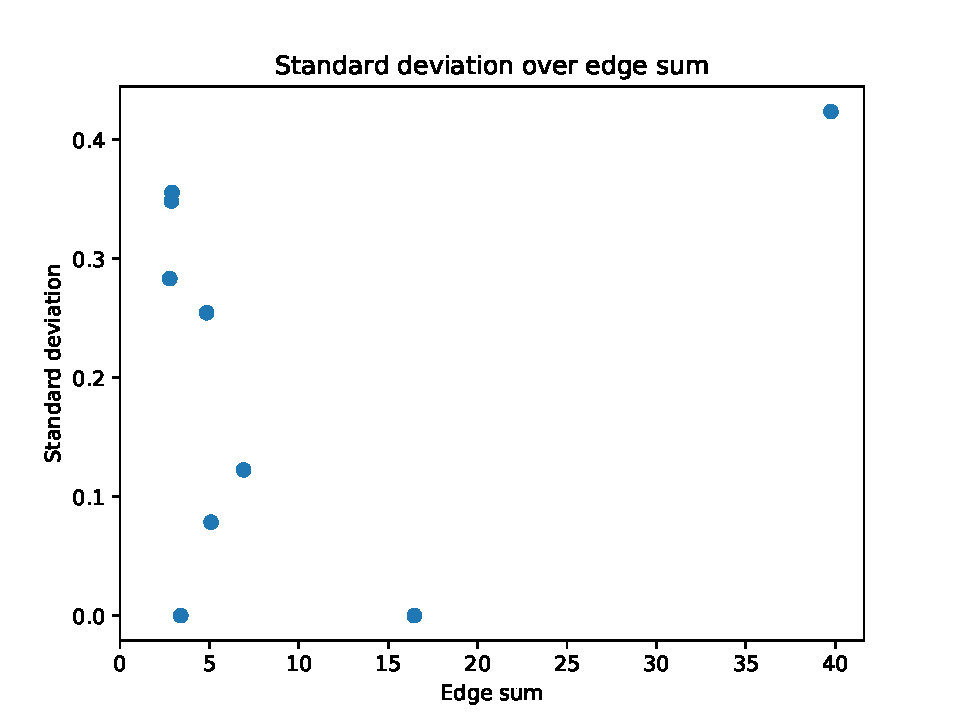
\includegraphics[width=\textwidth]{out/bbctech200/std-dev-edge-sum.pdf}
%                 \caption{@bbctech}
%                 \label{fig:out/bbctech200/std-dev-edge-sum.pdf}
%             \end{subfigure}
%             \begin{subfigure}[b]{0.4\textwidth}
%                 \centering
%                 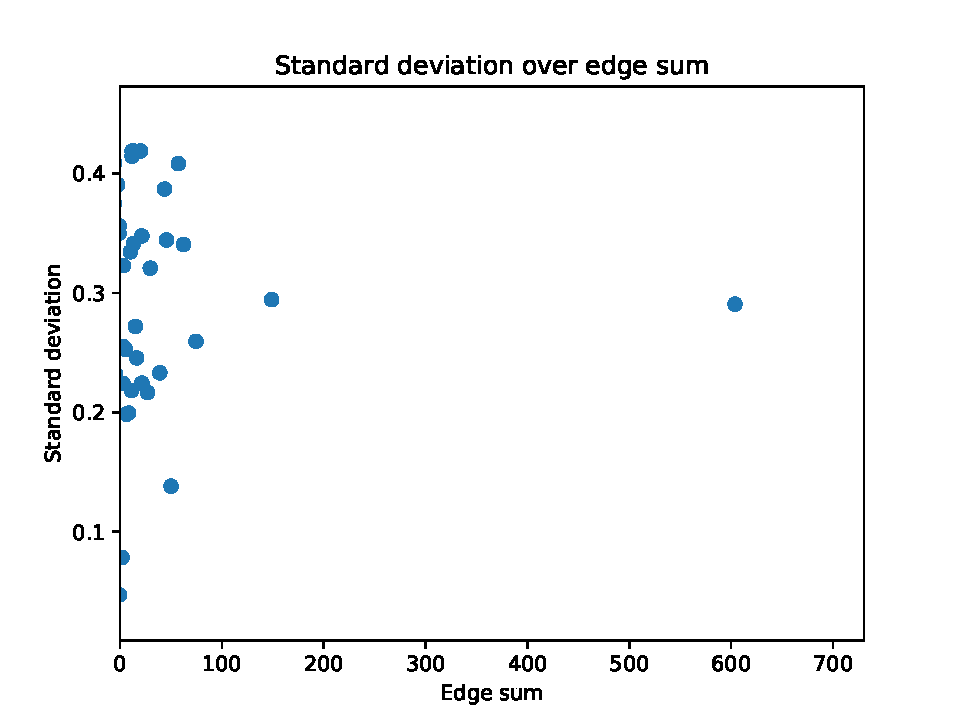
\includegraphics[width=\textwidth]{out/foxnews400/std-dev-edge-sum.pdf}
%                 \caption{@foxnews}
%                 \label{fig:out/foxnews400/std-dev-edge-sum.pdf}
%             \end{subfigure}
%             \begin{subfigure}[b]{0.4\textwidth}
%                 \centering
%                 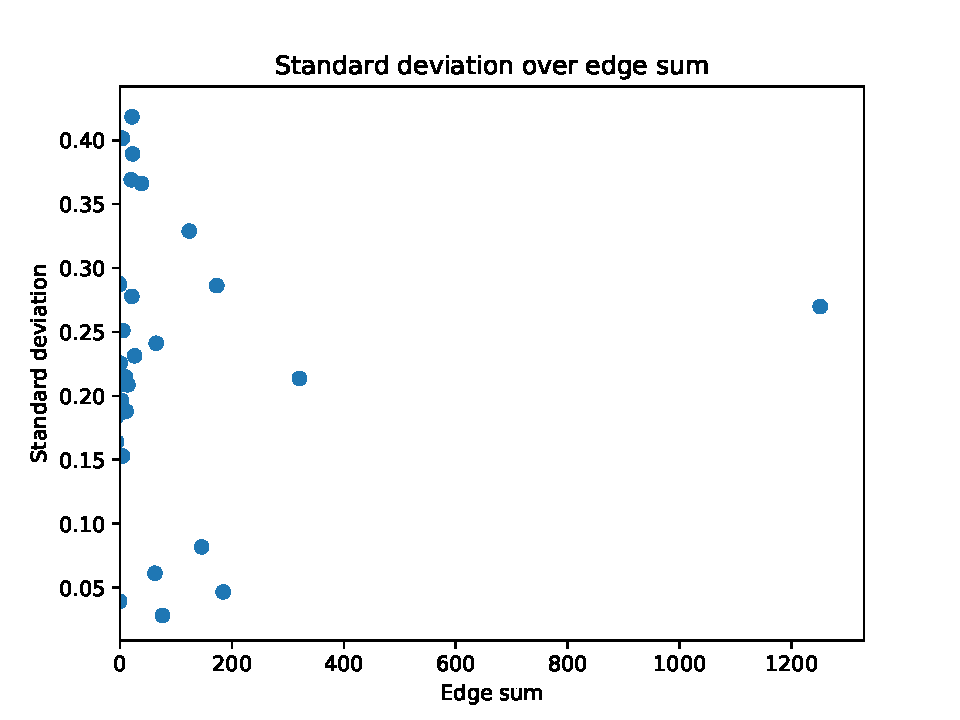
\includegraphics[width=\textwidth]{out/politics200/std-dev-edge-sum.pdf}
%                 \caption{r/politics}
%                 \label{fig:out/politics200/std-dev-edge-sum.pdf}
%             \end{subfigure}
%         \end{center}
%     \end{figure}
% \end{frame}

\begin{frame}[c]
    \frametitle{Detecting controversial content}

    \begin{itemize}
        \item Controversial content usually receives many more replies
        \item Another possibility for detecting it (needs to be verified)
            \begin{enumerate}
                \item select content $C$ with high standard deviation (of the
                    fraction of negative edges $\eta(C)$), which may be
                    associated with an higher number of interactions
                \item keep content $C$ whose $\eta(C) > \alpha $
            \end{enumerate}
    \end{itemize}
\end{frame}


\begin{frame}[c]
    \frametitle{The echo chamber problem - notation}
    \begin{itemize}
        \item $G = (V, E ^{+}, E ^{-}) $ interaction graph
        \item $ \mathcal{C} $ set of contents
        \item $C \in \mathcal{C} $ content, $\mathcal{T} _{C} $ set of threads
            associated with $C$. A thread $T \in \mathcal{T} _{C} $ is a
            subgraph of $G$
            % So $G = \bigcup _{C
            % \in \mathcal{C} } \bigcup _{T \in \mathcal{T} _C} T $ union of all
            % threads of all contents
        \item $U \subseteq V$ subset of users, $T[U]$ subgraph of $T$ induced
            by $U$. $|T(U)|$ is the number of edges of this subgraph
    \end{itemize}
\end{frame}

\begin{frame}[c]
    \frametitle{The echo chamber problem - notation}
    \begin{itemize}
        \item $\eta(C)$ fraction of negative edges associated with $C$
            (analogous definition for a thread $T$). Content (or thread)
            controversial if $\eta \in [\alpha, 1]$
        \item $\hat{\mathcal{C} } \subseteq \mathcal{C} $ set of \textit{controversial}
            contents

        \item $\mathcal{S} _C (U)$ set of \textit{non controversial} threads
            induced by $U$, for \textit{controversial} contents, i.e.

            {\small
                \begin{equation}
                    \mathcal{S} _{C} (U) = \{ T[U] \; s.t. \; T[U] \; non \;
                        controversial, T \in \mathcal{T} _{C}, C
                    \in \hat{\mathcal{C}}, U \subseteq V\}
                \end{equation}
            }
    \end{itemize}

\end{frame}

\begin{frame}[c]
    \frametitle{The echo chamber problem}
    \textbf{Goal}: given an interaction graph $G$, find $U \subseteq V$ maximing

    \begin{equation}
        \xi (U) = \sum^{}_{C \in \hat{\mathcal{C}} } \sum^{}_{T[U] \in S_C (U)}
        | T[U] |
    \end{equation}

    The set of users maximing the expression is denoted as $\hat{U}$ and the
    corresponding score is $\xi(G)$
\end{frame}

\begin{frame}[c]
    \frametitle{The datasets - negative edge fractions for contents}
    \begin{figure}
        \begin{center}
            \begin{subfigure}[b]{0.4\textwidth}
                \centering
                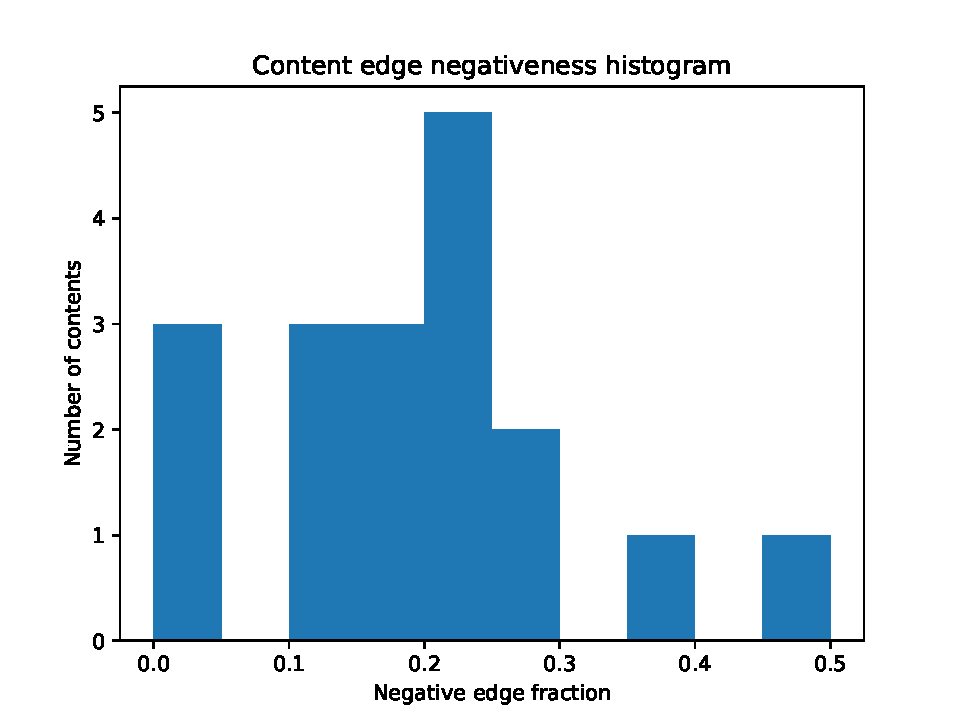
\includegraphics[width=\textwidth]{out/emanews200/neg-fraction-content-hist.pdf}
                \caption{@emanews}
                \label{fig:out/emanews200/neg-fraction-content-hist.pdf}
            \end{subfigure}
            \begin{subfigure}[b]{0.4\textwidth}
                \centering
                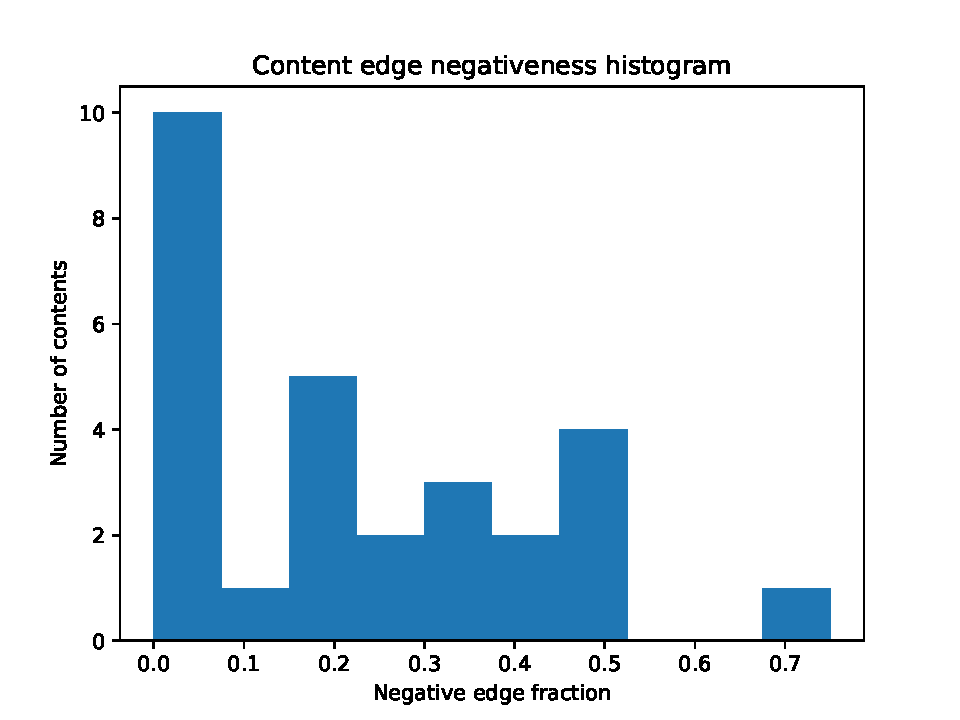
\includegraphics[width=\textwidth]{out/bbcscience200/neg-fraction-content-hist.pdf}
                \caption{@bbcscience}
                \label{fig:out/bbcscience200/neg-fraction-content-hist.pdf}
            \end{subfigure}
            \begin{subfigure}[b]{0.4\textwidth}
                \centering
                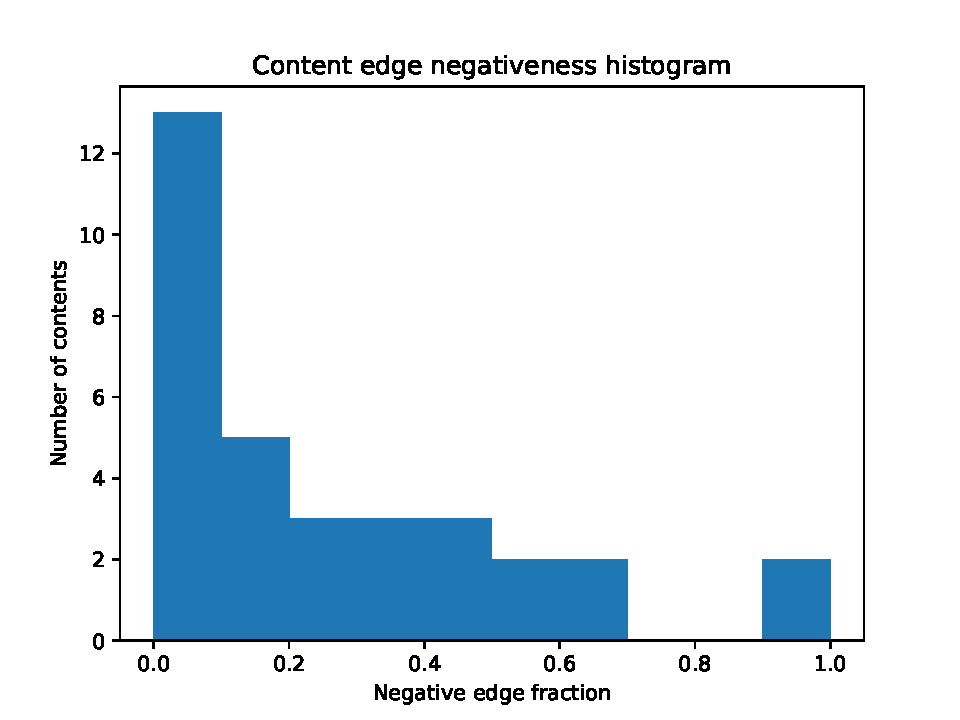
\includegraphics[width=\textwidth]{out/bbctech200/neg-fraction-content-hist.pdf}
                \caption{@bbctech}
                \label{fig:out/emanews200/neg-fraction-content-hist.pdf}
            \end{subfigure}
            \begin{subfigure}[b]{0.4\textwidth}
                \centering
                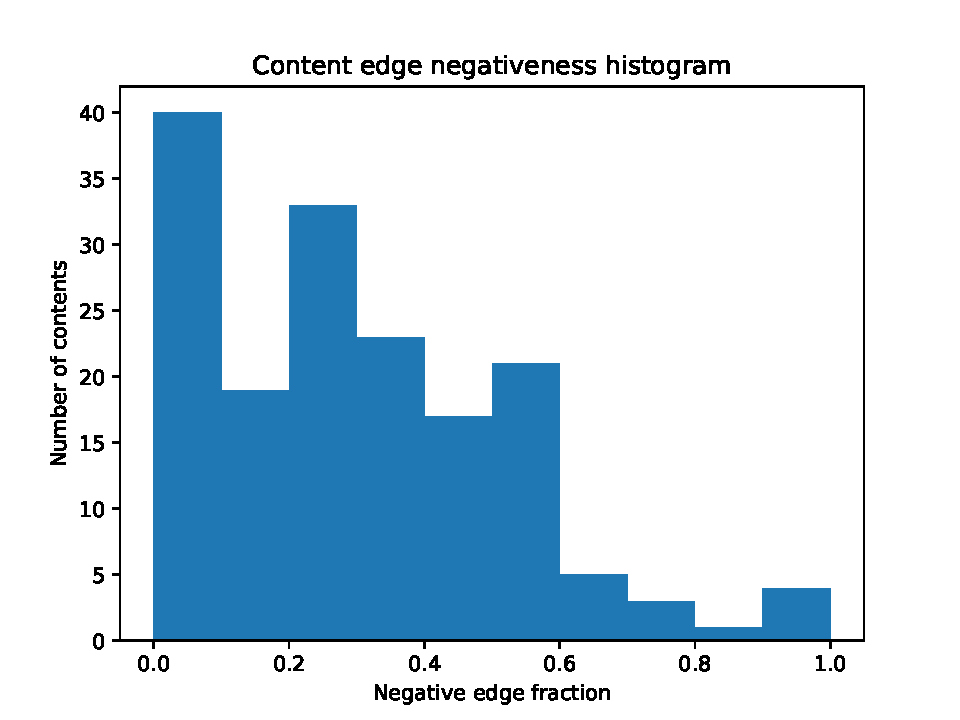
\includegraphics[width=\textwidth]{out/bbcsport200/neg-fraction-content-hist.pdf}
                \caption{@bbcsports}
                \label{fig:out/bbcscience200/neg-fraction-content-hist.pdf}
            \end{subfigure}
        \end{center}
    \end{figure}

\end{frame}

\begin{frame}[c]
    \frametitle{Echo chamber scores of connected components}
    \begin{table}[htpb]
        \centering
        \caption{Echo chamber scores, by components}
        \begin{tabular}{c|c|c|c|c|c}
            \textbf{Source} & {|V|} & {|E|} & {$\xi(G)$} &
            {|$\hat{U}$|} & $\xi(G)$/{|$\hat{U}|$} \\
            \hline
            @emanews & 1226 & 1842 & 0 & 0 & - \\
            @bbcscience & 447 & 388 & 4 & 2 & 0.5 \\
            @bbctech & 793 & 719 & 26 & 12 & 2.17 \\
            @bbcsports & 1645 & 2457 & 0 & 0 & - \\
        \end{tabular}
    \end{table}

    \begin{figure}[htpb]
        \centering
        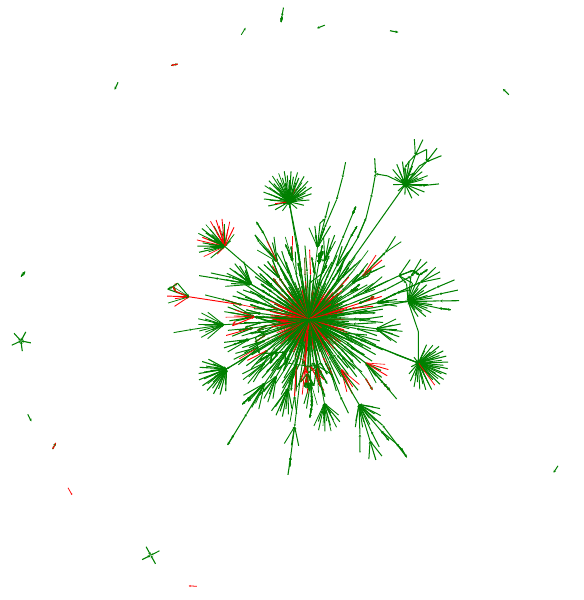
\includegraphics[width=0.3\linewidth]{img/graph.png}
        \label{fig:img/graph}
    \end{figure}

\end{frame}

\begin{frame}[c]
    \frametitle{An initial implementation}

    \begin{algorithm}[H]
        \SetAlgoLined
        % \KwResult{Write here the result }
        $U = \{$ random node $\}$\;
        \While{$\xi(U)$ can be increased by adding a node}{
            With probability $\beta $  {
                add to $U$ the node increasing more the score
                $\xi(U)$ (taking into account variations in $S_C (U)$)\;
            }
            With probability $(1 - \beta )$ remove from $U$ the node increasing less the
            score $\xi(U)$. This node will be ignored in the next iteration\;
        }
        \caption{Greedy approach}
    \end{algorithm}

    \begin{itemize}
        \item Process is repeated for many nodes and maximum score is selected
        \item Final score is divided by the number of nodes of the graph.
        \item Set of users is \textit{compacted} by the random node removal
        \item $\beta $  regulates $density$ of the user group
    \end{itemize}

\end{frame}

\begin{frame}[c]
    \frametitle{An initial implementation - results}
    Process was repeated $ \sqrt{n}$ times for a graph with $n$ nodes


    \begin{table}[htpb]
        \centering
        \caption{Echo chamber scores, greedy approach}
        \begin{tabular}{c|c|c|c|c|c|c}
            \textbf{Source} & {|V|} & {|E|} & $\beta $ & {$\xi(G)$} &
            {|$\hat{U}$|} & $\xi(G)$/{|$\hat{U}|$} \\
            \hline
            \multirow{5}{*}{@emanews} & \multirow{5}{*}{1226} & \multirow{5}{*}{1842} & 0.6 & 0 & 0 & - \\
                                      &  & & 0.7 & 0 & 0 & - \\
                                      &  & & 0.8 & 0 & 0 & - \\
                                      &  & & 0.9 & 0 & 0 & - \\
                                      &  & & 1 & 0 & 0 & - \\
        \end{tabular}
    \end{table}

\end{frame}

\begin{frame}[c]
    \frametitle{An initial implementation - results}
    \begin{table}[htpb]
        \centering
        \caption{Echo chamber scores, greedy approach}
        \begin{tabular}{c|c|c|c|c|c|c}
            \textbf{Source} & {|V|} & {|E|} & $\beta $ & {$\xi(G)$} &
            {|$\hat{U}$|} & $\xi(G)$/{|$\hat{U}|$} \\
            \hline
            \multirow{5}{*}{@bbcscience} & \multirow{5}{*}{447} &
            \multirow{5}{*}{388} & 0.6 & 2 & 2 & 1 \\
                                 &  & & 0.7 & 0 & 0 & - \\
                                 &  & & 0.8 & 6 & 3 & 2 \\
                                 &  & & 0.9 & 3 & 2 & 1.5 \\
                                 &  & & 1 & 2 & 3 & 0.67 \\
                                 \hline
            \multirow{5}{*}{@bbctech} & \multirow{5}{*}{793} &
            \multirow{5}{*}{719} & 0.6 & 28 & 9 & 3.11 \\
                                 &  & & 0.7 & 28 & 9 & 3.11 \\
                                 &  & & 0.8 & 28 & 9 & 3.11 \\
                                 &  & & 0.9 & 34 & 14 & 2.42 \\
                                 &  & & 1 & 28 & 9 & 3.11 \\
        \end{tabular}
    \end{table}
\end{frame}

\begin{frame}[c]
    \frametitle{An initial implementation - results}
    \begin{table}[htpb]
        \centering
        \caption{Echo chamber scores, greedy approach}
        \begin{tabular}{c|c|c|c|c|c|c}
            \textbf{Source} & {|V|} & {|E|} & $\beta $ & {$\xi(G)$} &
            {|$\hat{U}$|} & $\xi(G)$/{|$\hat{U}|$} \\
            \hline
            \multirow{3}{*}{@bbcsports} & \multirow{3}{*}{1645} &
            \multirow{3}{*}{2457} & 0.6 & 173 & 16 & 10.8 \\
                                  &  & & 0.7 & 159 & 12 & 13.25 \\
                                  &  & & 0.8 & 220 & 32 & 6.87 \\
                                  &  & & 0.9 & 224 & 36 & 6.22 \\
                                  &  & & 1 & 228 & 40 & 5.7 \\
        \end{tabular}
    \end{table}

    Note: algorithm was stopped at the 30th iteration.
\end{frame}

\begin{frame}[c]
    \frametitle{Another possible greedy approach}
    Inspired to the greedy algorithm proposed in
    \cite{10.1007/3-540-44436-X_10}

    \begin{algorithm}[H]
        \SetAlgoLined
        % \KwResult{Write here the result }
        $U = \{$ all nodes $\}$\;
        $S$ = $\xi(U)$ \;
        \While{$U$ is not empty}{
            remove from $U$ the node contributing less to the score $\xi(U)$\;
            update $S$ if the current score is higher\;
        }
        \caption{Greedy approach}
    \end{algorithm}

\end{frame}

% \begin{frame}[c]
%     \frametitle{Similarities between densest subgraph and echo chamber}
%     $U \subseteq V$, $E(U)$ edges induced by $U$
%
%     \bigskip
%
%     Densest subgraph problem
%
%     \begin{equation}
%         f(U)= \frac{|E(U)|}{|U|}
%     \end{equation}
%
%     Analogous \textit{normalized} echo chamber score
%
%     \begin{equation}
%         \xi' (U) = \sum^{}_{C \in \hat{\mathcal{C}} } \sum^{}_{T[U] \in S_C (U)}
%         \frac{| T[U] |}{|U|}
%     \end{equation}
%
% \end{frame}

\begin{frame}[c]
    \frametitle{Computing exactly the score}

    \begin{equation}
        maximize\; \sum^{}_{ij \in E(\hat{\mathcal{C}})} x _{ij}
    \end{equation}
    \begin{equation}
        x _{ij} \leq y_i \quad \forall ij \in E(\hat{\mathcal{C}})
    \end{equation}
    \begin{equation}
        x _{ij} \leq y_j \quad \forall ij \in E(\hat{\mathcal{C}})
    \end{equation}
    \begin{equation}
        \sum^{}_{ij \in E^{-} (T_k)} x_{ij} - \alpha \sum^{}_{ij \in E(T_k)}
        x_{ij} \leq M_k(1 -z_{k} ) \quad \forall T_{k} \in \mathcal{T} _{C}, C \in
        \mathcal{C}
    \end{equation}
    \begin{equation}
        \sum^{}_{ij \in E(T_{k} )} x_{ij} \leq N_{k} z_{k}
    \end{equation}
    \begin{equation}
        x _{ij} \in \{0, 1\} \quad \forall ij \in E(\hat{\mathcal{C}})
    \end{equation}
    \begin{equation}
        y _{i} \in  \{0, 1\} \quad \forall i \in V
    \end{equation}
    \begin{equation}
        z _{k} \in  \{0, 1\} \quad \forall T_{k} \in \mathcal{T} _{C}, C \in
        \mathcal{C}
    \end{equation}
\end{frame}

\begin{frame}[c]
    \frametitle{Computing exactly the score}
    A thread $T_{k} $ is non controversial if $\eta(T) \leq \alpha $, i.e.
    \begin{equation}
        \frac{\sum^{}_{ij \in e^{-} (t_{k} )} x_{ij} }
        {\sum^{}_{ij \in e^ (t_{k} )} x_{ij} } \leq \alpha
    \end{equation}

    which can be written as

    \begin{equation}
        \sum^{}_{ij \in e^{-} (t_{k} )} x_{ij} -
        \alpha {\sum^{}_{ij \in e^ (t_{k} )} x_{ij} } \leq 0
    \end{equation}

\end{frame}

\begin{frame}[c]
    \frametitle{Computing exactly the score}
    So, for controversial content

    \begin{equation}
        \sum^{}_{ij \in e^{-} (t_{k} )} x_{ij} -
        \alpha {\sum^{}_{ij \in e^ (t_{k} )} x_{ij} } > 0
    \end{equation}

    and, for the constraint
    \begin{equation}
        \sum^{}_{ij \in E^{-} (T_k)} x_{ij} - \alpha \sum^{}_{ij \in E(T_k)}
        x_{ij} \leq M_k(1 -z_{k} ) \quad \forall T_{k} \in \mathcal{T} _{C}, C \in
        \mathcal{C}
    \end{equation}

    it will be $z_{k} = 0$. So controversial $T_{k} \implies z_{k} = 0$.
\end{frame}

\begin{frame}[c]
    \frametitle{Computing exactly the score}
    \begin{equation}
        \sum^{}_{ij \in E(T_{k} )} x_{ij} \leq N_{k} z_{k}
    \end{equation}

    will set to $0$ edges associated to controversial threads $T_{k} $.

    So controversial $T_{k} \implies z_{k} = 0 \implies x_{ij} = 0 \quad \forall ij
    \in E(T_{k} )$.

\end{frame}

\begin{frame}[c]
    \frametitle{Computing exactly the score}
    $N_{k} $ and $M_{k} $ can be simply $m$, the number of edges in the graph.
\end{frame}

\begin{frame}[c]
    \frametitle{Bibliography}
    \printbibliography
\end{frame}
\end{document}


